% SC3010 --- Chapter 8: Applications: Privacy, Forensics, Response, Law (0->100 ground-up)
% No \documentclass --- this file is \input/\include'd by main.tex.
\chapter{Applications: Privacy, Forensics, Incident Response, and Law}
\label{ch:applications}
\begin{quote}
\emph{``Security is not only cryptography and firewalls; it is what happens when things fail, how we prove what happened, and what the law requires us to do.''} --- This chapter connects technical mechanisms to privacy guarantees, evidence, operations, and regulation.
\end{quote}
\noindent\fbox{\parbox{\dimexpr\linewidth-2\fboxsep-2\fboxrule}{%
\textbf{From zero: we build here, no law or statistics course needed.} We assume only that you have collected or seen data tables (rows = people, columns = attributes) and that organisations must respond when systems break. From those everyday starting points we formalise privacy, forensics, response, and GDPR obligations---pictures before definitions.}}
\vspace{0.4em}
\section*{Learning Outcomes}
After this chapter you will be able to:
\begin{enumerate}[label=(L\arabic*)]
    \item define $k$-anonymity, its limitations, and $l$-diversity/$t$-closeness refinements;
    \item state $\varepsilon$-differential privacy and apply the Laplace mechanism;
    \item explain chain-of-custody and forensically sound handling of digital evidence;
    \item describe the NIST incident-response lifecycle and map actions to each phase;
    \item summarise GDPR principles, lawful bases, data-subject rights, and breach-notification duties.
\end{enumerate}
% ============================================================
\section{Privacy: From Removing Names to Formal Guarantees}
\label{sec:privacy-intro}
Removing names is not anonymisation. Latanya Sweeney showed 87\% of Americans can be re-identified by \{ZIP, birthdate, gender\} alone---\emph{quasi-identifiers} combine with public voter rolls to single out a row. AOL search-log and Netflix Prize de-anonymisations repeat the lesson: linkage attacks defeat naive scrubbing.
We thus distinguish: \emph{identifier} (name, NRIC, email---directly identifying), \emph{quasi-identifier} (ZIP, age, gender---identifying in combination), and \emph{sensitive attribute} (disease, salary) we wish to protect.
% --- TikZ 1: k-anonymity ---
\begin{figure}[h]
\centering
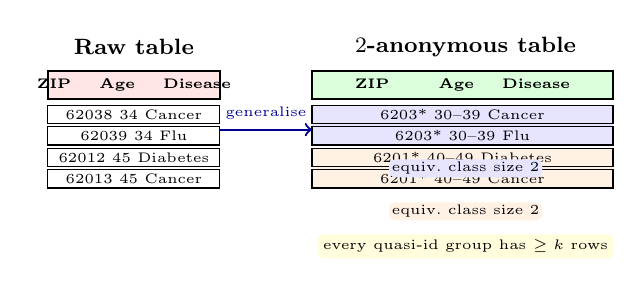
\begin{tikzpicture}[scale=0.78, every node/.style={font=\scriptsize}]
% Raw table
\node[font=\footnotesize\bfseries] at (-3.8,2.0) {Raw table};
\draw[thick,fill=red!10] (-5.2,1.6) rectangle (-2.4,1.15) node[midway,font=\tiny\bfseries] {ZIP \quad Age \quad Disease};
\foreach \y/\txt in {0.85/62038 34 Cancer,0.50/62039 34 Flu,0.15/62012 45 Diabetes,-0.20/62013 45 Cancer} {
  \draw[fill=white] (-5.2,\y+0.20) rectangle (-2.4,\y-0.10) node[midway,font=\tiny] {\txt};
}
\draw[->,thick,blue!60!black] (-2.4,0.65) -- (-0.9,0.65) node[midway,above,font=\tiny] {generalise};
% k-anonymous table
\node[font=\footnotesize\bfseries] at (1.6,2.0) {$2$-anonymous table};
\draw[thick,fill=green!14] (-0.9,1.6) rectangle (4.0,1.15) node[midway,font=\tiny\bfseries] {ZIP \qquad Age \quad Disease};
\fill[blue!10] (-0.9,0.85+0.20) rectangle (4.0,0.50-0.10);
\fill[orange!10] (-0.9,0.15+0.20) rectangle (4.0,-0.20-0.10);
\foreach \y/\txt in {0.85/6203* 30--39 Cancer,0.50/6203* 30--39 Flu,0.15/6201* 40--49 Diabetes,-0.20/6201* 40--49 Cancer} {
  \draw (-0.9,\y+0.20) rectangle (4.0,\y-0.10) node[midway,font=\tiny] {\txt};
}
\node[font=\tiny,fill=blue!10,rounded corners=2pt,inner sep=1pt] at (1.6,0.02) {equiv.\ class size $2$};
\node[font=\tiny,fill=orange!10,rounded corners=2pt,inner sep=1pt] at (1.6,-0.68) {equiv.\ class size $2$};
\node[font=\tiny,align=center,fill=yellow!14,rounded corners=2pt,inner sep=2pt] at (1.6,-1.25) {every quasi-id group has $\ge k$ rows};
\end{tikzpicture}
\caption{Generalisation to achieve $k$-anonymity ($k=2$): ZIP truncated and ages bucketed so each quasi-identifier tuple appears at least $k$ times. Suppression ($*$) trades utility for indistinguishability.}
\label{fig:k-anon}
\end{figure}
\begin{definition}[$k$-anonymity]
A table satisfies \emph{$k$-anonymity} if every combination of quasi-identifier values appears in at least $k$ rows. Each such group is an \emph{equivalence class}.
\end{definition}
Mechanisms: \emph{generalisation} (replace 62038 with 6203*, 34 with 30--39) and \emph{suppression} (delete outlier rows). Trade-off: larger $k$ means stronger indistinguishability but coarser data.
\begin{example}[Homogeneity attack]
A $2$-anonymous class \{(\texttt{6203*}, 30--39): Cancer, Cancer\} is $2$-anonymous yet reveals the sensitive value---everyone in the class has Cancer. $k$-anonymity does not protect attribute disclosure.
\end{example}
Refinements: \emph{$l$-diversity} requires each class to contain at least $l$ well-represented sensitive values; \emph{$t$-closeness} requires the distribution of the sensitive attribute in each class to be within distance $t$ of the global distribution. None is composable or robust to background knowledge---hence the move to differential privacy.
% ============================================================
\section{Differential Privacy}
\label{sec:dp}
\emph{Differential privacy} (DP) gives a mathematical promise about an \emph{algorithm}, not a static table: its output distribution barely changes if one person's row changes. The adversary may know all other rows.
\begin{definition}[$\varepsilon$-DP]
A randomised mechanism $\mathcal{M}$ is \emph{$\varepsilon$-differentially private} if for all neighbouring datasets $D,D'$ differing in one row and all output sets $S$,
\[ \Pr[\mathcal{M}(D)\in S] \;\le\; e^{\varepsilon}\,\Pr[\mathcal{M}(D')\in S]. \]
Smaller $\varepsilon$ means stronger privacy; typically $\varepsilon\in[0.1,5]$.
\end{definition}
Intuition: the factor $e^{\varepsilon}\approx1+\varepsilon$ for small $\varepsilon$ bounds how much one person can influence the output---plausible deniability. DP composes: $k$ $\varepsilon_i$-DP releases together are $(\sum\varepsilon_i)$-DP (basic composition); privacy budget must be managed.
\paragraph{Laplace mechanism.} For a numeric query $f$ with \emph{global sensitivity} $\Delta f=\max_{D\sim D'}|f(D)-f(D')|$, adding Laplace noise scaled to $\Delta f/\varepsilon$ yields $\varepsilon$-DP.
\[ \mathcal{M}(D)=f(D)+Y,\qquad Y\sim\mathrm{Lap}(\Delta f/\varepsilon),\quad p_Y(y)=\tfrac{\varepsilon}{2\Delta f}e^{-\varepsilon|y|/\Delta f}. \]
Counting queries have $\Delta f=1$; summing salaries has sensitivity equal to max salary range.
\begin{lstlisting}[language=Python]
import numpy as np
def laplace_mech(true_answer, sensitivity, epsilon):
    scale = sensitivity / epsilon          # larger epsilon -> less noise
    noise = np.random.laplace(0, scale)
    return true_answer + noise
# Example: count of patients with disease; sensitivity=1, epsilon=0.5
noisy_count = laplace_mech(42, sensitivity=1, epsilon=0.5)
\end{lstlisting}
% --- TikZ 2: DP noise illustration ---
\begin{figure}[h]
\centering
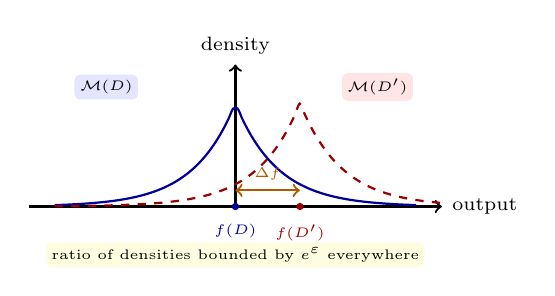
\begin{tikzpicture}[scale=0.82, every node/.style={font=\scriptsize}]
\draw[->,thick] (-3.2,0) -- (3.2,0) node[right] {output};
\draw[->,thick] (0,0) -- (0,2.2) node[above] {density};
% Two Laplace densities centred at 0 and 1
\draw[thick,blue!60!black,smooth,domain=-2.8:2.8,samples=80] plot (\x,{1.6*exp(-abs(\x)/0.65)});
\draw[thick,red!60!black,dashed,smooth,domain=-2.8:3.2,samples=80] plot (\x,{1.6*exp(-abs(\x-1)/0.65)});
\fill[blue!60!black] (0,0) circle (1.6pt) node[below=3pt,font=\tiny] {$f(D)$};
\fill[red!60!black] (1,0) circle (1.6pt) node[below=3pt,font=\tiny] {$f(D')$};
\node[font=\tiny,fill=blue!10,rounded corners=2pt,inner sep=2pt] at (-2.0,1.85) {$\mathcal{M}(D)$};
\node[font=\tiny,fill=red!10,rounded corners=2pt,inner sep=2pt] at (2.2,1.85) {$\mathcal{M}(D')$};
\draw[<->,thick,orange!70!black] (0,0.25) -- (1,0.25) node[midway,above,font=\tiny] {$\Delta f$};
\node[font=\tiny,align=center,fill=yellow!12,rounded corners=2pt,inner sep=2pt] at (0,-0.75) {ratio of densities bounded by $e^{\varepsilon}$ everywhere};
\end{tikzpicture}
\caption{Differential privacy: neighbouring datasets induce nearby output distributions (Laplace here). No output is much more likely under $D$ than under $D'$.}
\label{fig:dp-noise}
\end{figure}
Local vs.\ central DP, $(\varepsilon,\delta)$-DP relaxations, and composition accounting (moments accountant) extend the model; randomised response is the local-DP analogue for surveys.
% ============================================================
\section{Digital Forensics and Chain-of-Custody}
\label{sec:forensics}
When a breach becomes a legal matter, \emph{digital forensics} must answer what happened in a way a court can trust. The process is: \emph{identify} $\to$ \emph{preserve} $\to$ \emph{collect} $\to$ \emph{examine} $\to$ \emph{analyse} $\to$ \emph{report}, with integrity at every step.
\paragraph{Forensically sound handling.} Work on a \emph{bit-for-bit image}, never the original; attach a write blocker; hash immediately (SHA-256) and re-hash at every transfer to prove the image has not changed. Document tool versions and commands so another analyst can reproduce the result.
\paragraph{Chain-of-custody.} A chronological, signed record of who handled the evidence, when, why, and what was done. Gaps or undocumented access render evidence inadmissible---even a perfect forensic image is worthless if you cannot prove it is the image of the seized disk. Store hashes and custody forms separately from the evidence; timestamp with a trusted source.
\paragraph{Order of volatility (RFC~3227).} Collect most ephemeral first: registers/cache $\to$ RAM $\to$ network state $\to$ running processes $\to$ disk $\to$ backups/archives. Pulling the power preserves disk but destroys RAM artefacts (in-memory malware, decryption keys); live acquisition may be required but must be justified and logged.
\begin{lstlisting}[language=Python]
# forensically sound imaging (conceptual)
import hashlib
def image_and_hash(src_path, dst_path):
    h = hashlib.sha256()
    with open(src_path, 'rb') as src, open(dst_path, 'wb') as dst:
        while chunk := src.read(1<<20):  # 1 MiB at a time
            h.update(chunk); dst.write(chunk)
    digest = h.hexdigest()
    log(f"SHA-256({dst_path})={digest}  tool=v1.2  examiner=Alice  time=2026-08-28T09:00Z")
    return digest
# Re-hash before analysis; mismatch -> custody failure
\end{lstlisting}
Anti-forensics (timestomping, log wiping, steganography) must be anticipated; corroborate across independent sources (disk, netflow, cloud audit logs).
% ============================================================
\section{Incident Response: The NIST Lifecycle}
\label{sec:ir}
Incident response (IR) is the operational discipline of handling breaches. NIST SP~800-61 Rev.~2 organises it into four phases forming a cycle:
% --- TikZ 3: NIST lifecycle ---
\begin{figure}[h]
\centering
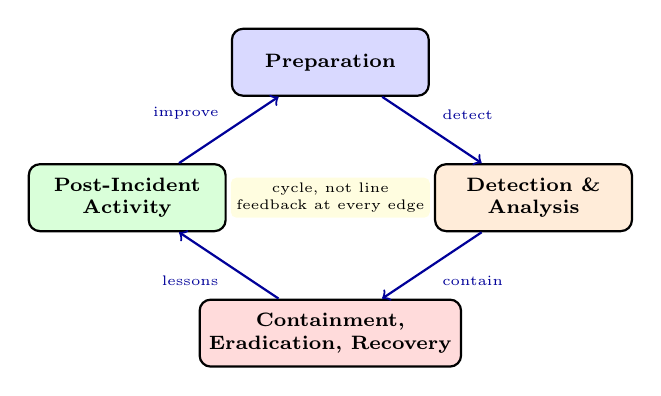
\begin{tikzpicture}[scale=0.86, every node/.style={font=\scriptsize},
  phase/.style={draw,thick,rounded corners=4pt,minimum width=2.5cm,minimum height=0.85cm,align=center}]
\node[phase,fill=blue!15] (prep) at (0,2.0) {\textbf{Preparation}};
\node[phase,fill=orange!15] (detect) at (3.0,0) {\textbf{Detection \&}\\ \textbf{Analysis}};
\node[phase,fill=red!14] (contain) at (0,-2.0) {\textbf{Containment,}\\ \textbf{Eradication, Recovery}};
\node[phase,fill=green!15] (post) at (-3.0,0) {\textbf{Post-Incident}\\ \textbf{Activity}};
\draw[->,thick,blue!60!black] (prep) -- (detect) node[midway,above right,font=\tiny] {detect};
\draw[->,thick,blue!60!black] (detect) -- (contain) node[midway,below right,font=\tiny] {contain};
\draw[->,thick,blue!60!black] (contain) -- (post) node[midway,below left,font=\tiny] {lessons};
\draw[->,thick,blue!60!black] (post) -- (prep) node[midway,above left,font=\tiny] {improve};
% inner note
\node[font=\tiny,align=center,fill=yellow!12,rounded corners=2pt,inner sep=2pt] at (0,0) {cycle, not line\\feedback at every edge};
\end{tikzpicture}
\caption{NIST incident-response lifecycle: preparation enables every other phase; post-incident feeds back into preparation.}
\label{fig:nist-ir}
\end{figure}
\paragraph{1.~Preparation.} Policies, playbooks, asset inventories, logging/monitoring, IR team roles (technical, legal, comms), tabletop exercises. Without preparation the other phases improvise.
\paragraph{2.~Detection \& Analysis.} Triage alerts (IDS, EDR, SIEM), scope the incident, preserve evidence forensically, assign severity. Key question: is this an \emph{event} or an \emph{incident} (adverse impact)?
\paragraph{3.~Containment, Eradication \& Recovery.} \emph{Short-term} containment (isolate host, block IP) stops bleeding; \emph{long-term} containment hardens. Eradicate root cause (remove backdoor, patch, rotate creds). Recover by restoring from known-good backups and monitoring for resurgence. Every action is logged for custody and later review.
\paragraph{4.~Post-Incident Activity.} Lessons-learned meeting, root-cause analysis, metrics (MTTD/MTTR), update playbooks and controls. The output is a report that improves Preparation---closing the loop.
Prioritisation uses impact vs.\ recoverability; communication plans separate internal, customer, regulator, and public messaging to avoid contradictory disclosures.
% ============================================================
\section{Regulation: GDPR Essentials}
\label{sec:gdpr}
The EU General Data Protection Regulation (2016/679) applies to any organisation processing personal data of EU residents, regardless of where the organisation sits. Key ideas:
\paragraph{Principles (Art.~5).} Lawfulness, fairness, transparency; purpose limitation; data minimisation; accuracy; storage limitation; integrity/confidentiality; accountability (you must \emph{demonstrate} compliance).
\paragraph{Lawful bases (Art.~6).} Processing needs one of six bases: consent, contract, legal obligation, vital interests, public task, or legitimate interests (balanced against rights). Consent must be freely given, specific, informed, unambiguous, and withdrawable.
\paragraph{Roles.} \emph{Data subject} (person), \emph{data controller} (decides purposes/means), \emph{data processor} (acts for controller), \emph{DPO} and \emph{supervisory authority}.
\paragraph{Rights of the data subject.} Access, rectification, erasure (``right to be forgotten''), restriction, portability, objection, and not to be subject to solely automated decision-making (Art.~12--22).
\paragraph{Obligations \& breach notification.} Data Protection Impact Assessments for high-risk processing, records of processing, security by design/default (Art.~25, 32). Breach notification to the authority within \textbf{72~hours} of awareness (Art.~33) and to affected subjects without undue delay if high risk (Art.~34). Fines up to \texteuro20m or 4\% of global annual turnover, whichever is higher.
Other regimes (Singapore PDPA, US sectoral laws, CCPA/CPRA) differ in scope and enforcement but share the trajectory: minimise data, justify retention, notify promptly, and be auditable.
% ============================================================
\section{Budget, Custody, and Notification: A Worked Scenario}
\label{sec:putting-together}
A mid-size SaaS company runs a containerised analytics platform. Three vignettes show how the chapters connect.
\paragraph{Vignette A: privacy budget.} The product team wants to publish daily counts of active users by region and by plan tier over a month (60 queries). Each is $\varepsilon=0.2$-DP via Laplace. Basic composition gives total $\varepsilon=12$---too large (almost no guarantee). Using advanced composition or splitting $\varepsilon$ to $0.05$ per query and adding a little more noise, or publishing only weekly aggregates, brings the monthly budget back under $\varepsilon=3$. The lesson: privacy, like incident response, needs budgeting before release, not after.
\paragraph{Vignette B: forensics meets IR.} An attacker exploits a container escape (mounted Docker socket, as in E7.5) and wipes \texttt{/var/log/auth.log}. Because the IR playbook mandated centralised, append-only log shipping and hourly disk images with SHA-256 chain-of-custody, the team reconstructs the attack from the SIEM and the previous image. Without custody, the wiped log would have been taken as ground truth.
\paragraph{Vignette C: GDPR clock.} Forensics confirms the attacker exfiltrated a user table that included EU residents. The 72-hour clock under Art.~33 started when the controller had ``reasonable degree of certainty'' (forensic confirmation), not when the IDS first fired. The controller notifies the supervisory authority within the window, documents the delay rationale, and notifies high-risk data subjects after scoping---exactly the post-incident reporting envisaged by NIST.
Together the three vignettes illustrate a single principle: technical guarantees (DP, isolation), operational discipline (forensics, IR), and legal duties (GDPR) must be designed jointly, because a failure in one undermines the others.
\begin{theorem}[Composition and utility trade-off]
Let $\mathcal{M}_1,\dots,\mathcal{M}_k$ each be $\varepsilon_i$-DP. Then the sequential release $(\mathcal{M}_1,\dots,\mathcal{M}_k)$ is $(\sum_i\varepsilon_i)$-DP. Reducing each $\varepsilon_i$ improves privacy but increases noise variance $\propto(\Delta f/\varepsilon_i)^2$, degrading utility. Choosing $\varepsilon$ is thus a policy decision balancing re-identification risk against data usefulness, and must be audited alongside GDPR data-minimisation.
\end{theorem}
\begin{example}[GDPR meets DP]
A hospital wants to publish average length-of-stay by diagnosis. Instead of releasing $k$-anonymous microdata (vulnerable to linkage via rare diagnoses), it releases Laplace-noised averages with $\varepsilon=1.0$ and documents the privacy budget in its Record of Processing Activities (RoPA). This satisfies purpose limitation and minimisation while giving a formal guarantee the supervisory authority can audit---a concrete bridge from mathematics to compliance.
\end{example}
\begin{remark}[Forensics readiness]
Logging with hash-chained integrity (e.g., \texttt{syslog} + RFC~3161 timestamps) and hardware-rooted attestation (TPM-measured boot) turns post-incident reconstruction from guesswork into checkable evidence. Readiness is cheaper than retroactive collection and is explicitly encouraged by GDPR Art.~32 (integrity and resilience).
\end{remark}
\begin{example}[Checklist: 72-hour clock]
Hour 0: IDS alert $\to$ SOC creates ticket, preserves RAM/disk images with hashes.
Hour 4: Forensic analysis confirms personal data exfiltration $\to$ awareness for Art.~33.
Hour 12: DPO drafts notification (nature, categories, approximate subjects, consequences, mitigation).
Hour 48: Authority notified; if risk is high, affected subjects notified directly.
Hour 72: Deadline for authority notification; document reasoning if any delay.
Every step is logged in the chain-of-custody register so the supervisory authority can audit timeliness and completeness.
\end{example}
\begin{remark}[Singapore contrast]
Singapore's PDPA also requires breach notification (since 2021) but with a 3-calendar-day window to the PDPC and notification to affected individuals if significant harm is likely. Comparing timelines shows why multinationals map a single playbook to the strictest deadline---GDPR's 72 hours---and add local annexes.
\end{remark}
% ============================================================
\section{Exercises}
\label{sec:ch08-exercises}
\begin{enumerate}[label=E8.\arabic*, leftmargin=*, itemsep=0.6em]
    \item \textbf{$k$-anonymity construction.} Table has quasi-identifiers \{ZIP, Age\} and sensitive Disease. Generalise ZIP to 3 digits and bucket ages into 10-year intervals to achieve $k=3$. Show the resulting equivalence classes. Give a homogeneity attack on your table and explain how $l$-diversity would block it.
    \item \textbf{Differential privacy calculation.} A counting query has sensitivity $\Delta f=1$ and mechanism $M(D)=f(D)+\mathrm{Lap}(1/\varepsilon)$ with $\varepsilon=0.5$. Compute $\Pr[|M(D)-f(D)|>2]$ and the factor $e^{\varepsilon}$ bounding neighbouring likelihood ratios. If you answer 10 such queries with basic composition, what is the total $\varepsilon$?
    \item \textbf{Chain-of-custody failure.} An analyst images a disk, forgets to hash it, edits the image to extract a file, then hashes. Opposing counsel moves to exclude the evidence. Explain why the chain is broken, what the correct forensically sound workflow is, and how order of volatility should have guided collection if RAM contained the decryption key.
    \item \textbf{NIST lifecycle tabletop.} A ransomware alert fires at 02:00 on a file server. Map the next 48 hours to the four NIST phases, listing concrete tasks, owners (SOC, IT, legal, comms), and evidence-preservation steps. Where does the 72-hour GDPR clock fit?
    \item \textbf{GDPR analysis.} A Singapore e-commerce site tracks EU visitors' browsing via cookies for ads (a) without consent and (b) with a pre-ticked box. Identify the lawful basis (if any), which GDPR principles are violated, which data-subject rights are engaged, and the breach-notification duty if the cookie database leaks.
\end{enumerate}
% ============================================================
\section*{Chapter Notes}
Privacy: Sweeney (2002) $k$-anonymity; Machanavajjhala et al.\ (2007) $l$-diversity; Li et al.\ (2007) $t$-closeness; Dwork et al.\ (2006) differential privacy, Laplace mechanism; Dwork \& Roth (2014) survey. Forensics: Carrier (2005), RFC~3227 volatility, NIST SP~800-86. Incident response: NIST SP~800-61 Rev.~2, MITRE ATT\&CK for detection mapping. GDPR: Regulation 2016/679; see Art.~5, 6, 12--22, 25, 32--34; Singapore PDPA (2012, rev.\ 2020) for contrast; EDPB guidelines on consent and breach notification.
% End of Chapter 8
